\documentclass[ ../main.tex]{subfiles}
\providecommand{\mainx}{..}
\begin{document}
\section{False negative rate}
The perfect hash map can represent false positives in the understood way.

However, if we fix the size of the entropy bits per element in the domain of definition, false negatives arise in a natural way. Suppose we fix the entropy at $d$ bits and we have some value type that has a prefix free encoding.

We consider the simplest one first, where each value has one or more representations of fixed bit length $k$.

For a given element $x$ with a value $y = \Fun{f}(x)$ with $\Fun{n}(y)$ representations, the probability that a random hash $\Fun{h}(j)$, $j \in \BitSet^d$, maps to one of the $\Fun{n}(y)$ representations is $p = \Fun{n}(y) / 2^k$.


We have $2^d$ hash values in $\BitSet^d$ we may try. Each trial for a given element is independent and geometrically distributed $\geodist(p)$.

The first match is expected to take $\frac{1}{p} = \frac{2^k}{\Fun{n}(y)}$ trials.
The probability that no hash value will be found in $\BitSet^d$ that matches one of the representations of $\Fun{n}(y)$ is $q^{2^d}$ where $q = 1 - p = 1-\frac{\Fun{n}(y)}{2^k}$.

The simplest case is $\Fun{n}(y) = 1$, then the probability $\left(1-2^{-k}\right)^{2^d}$.
At the limit, as $d \to \infty$, the probability that no match will be found goes to zero as illustrated by figure~1.

%\begin{tikzpicture}
%\pgfmathdeclarefunction{f}{1}{%
%	\pgfmathparse{abs(1-(1-((#1+1)/2)^2)^(#1))^(#1)}%
%}%
%\begin{axis}[
%axis lines = left,
%%xmin    = 20,
%%xmax    = 30,
%%ymin    = 0,
%%ymax    = 1,
%xlabel  = $d$,
%ylabel  = {$\Fun{n}(y)$}
%]
%%Below the red parabola is defined
%\addplot[domain=0:16,samples=100]()
%{
%	f(x)
%};
%%\addlegendentry{$(1-2^{-16})^{2^d}$}
%\end{axis}
%\end{tikzpicture}

We may solve for any probability of no match by choosing an appropriate $\Fun{n}(y)$.



Solving for $\Fun{n}(y)$, we transform the above by the sequence of transformations
\begin{align}
\left(1-\frac{\Fun{n}(y)}{2^k}\right)^{2^d}
&= \alpha\\
1-\frac{\Fun{n}(y)}{2^k}  	&= \alpha^{\frac{1}{2^d}}\\
\frac{\Fun{n}(y)}{2^k}    	&= 1 - \alpha^{\frac{1}{2^d}}\\
\Fun{n}(y)                	&= 2^k\left(1 - \alpha^{2^{-d}}\right)\,.
\end{align}

with the constraint that $\sum_{y \in } \Fun{n}(y)$ 


Thus, given a fixed size $k$ of 



--------





The perfect hash map can represent false positives in the understood way.

However, if we fix the size of the entropy bits per element in the domain of definition, false negatives arise in a natural way.
Suppose we fix the entropy at $d$ bits and we have some value type that has a prefix free encoding.

We consider the simplest one first, where each value has one or more representations of fixed bit length $k$.
For a given element $x$ with a value $y = f(x)$ with $n_y$ representations, the probability that a random hash $\Fun{h}(j)$, $j \in \{0,1\}^d$, maps to one of the $n_y$ representations is $p = n_y / 2^k$.
We have $2^d$ hash values in $\{0,1\}^d$ we may try where each trial for a given element is independent and geometrically distributed $\textrm{GEO}(p)$.

The first match is expected to take $\frac{1}{p} = \frac{2^k}{n_y}$ trials.
The probability that hash value will be found in $\{0,1\}^d$ that matches one of the representations of $n_y$ is $q^{2^d}$ where $q = 1 - p = 1-\frac{n_y}{2^k}$.

The simplest case is $n_y = 1$, then the probability $\fnrate = (1-2^{-k})^{2^d}$.
At the limit, as $d \to \infty$, $\fnrate$ goes to zero as illustrated by fig~1.

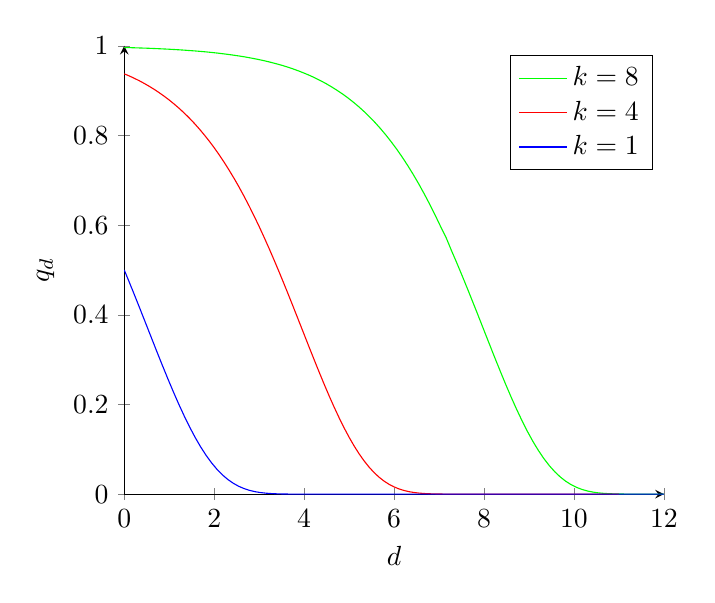
\begin{tikzpicture}
\begin{axis}[
    axis lines = left,
	ymin    = 0,
    ymax    = 1,
    xlabel  = $d$,
    ylabel  = {$q_d$}
]
\addplot[color=green,domain=0:12,samples=100]
{
    (1-2^(-8))^(2^\x)
};
\addlegendentry{$k=8$}
\addplot[color=red,domain=0:11,samples=100]
{
	(1-2^(-4))^(2^\x)
};
\addlegendentry{$k=4$}
\addplot[color=blue,domain=0:12,samples=100]
{
	(1-2^(-1))^(2^\x)
};
\addlegendentry{$k=1$}
\end{axis}
\end{tikzpicture}


We may solve for $d$ in $q(d) = \fnrate$ for any given $\fnrate \in (0,1)$ and $k$.
\begin{equation}
q_d = (1-2^{-k})^{2^d}
\end{equation}


We may solve for any probability of no match by choosing an appropriate $n(y)$.

\begin{theorem}
Given entropy $d$ and false negative rate $\fnrate$ codes of fixed-length $k$, the number of representations per $y \in \Set{Y}$ is given by
\begin{equation}
    n_y = 2^k\left(1 - \fnrate^{2^{-d}}\right)\,.
\end{equation}    
\end{theorem}
\begin{proof}
By \cref{dummy},
\begin{equation}
	\fnrate = \left(1-\frac{n_y}{2^k}\right)^{2^d}\,.
\end{equation}
Solving for $n_y$, we transform the above by the sequence of transformations
\begin{align}
    \left(1-\frac{n_y}{2^k}\right)^{2^d}
                       &= \fnrate\\                       
    1-\frac{n_y}{2^k}  &= \sqrt[2^d]{\fnrate}\\
    \frac{n_y}{2^k}    &= 1 - \sqrt[2^d]{\fnrate}\\
    n_y                &= 2^k\left(1 - \sqrt[2^d]{\fnrate}\right)\,.
\end{align}
\end{proof}





----


Suppose there are $N$ values of type $Y$ for approximate hash maps of type $X \mapsto Y$.\footnote{Technically, we could use the \emph{range} of the hash map, but the codomain is generally more appropriate to consider, especially in the case of \emph{cipher} hash maps.}

If we assume each 
TODO: mention that $2^k$ is worst-case limit for a prefix free code. If all equally probable, $2^k$ is ideal

If we fix $d$ instead of increasing it as necessary, we have a situation in which \emph{no matches} may be found.
We also have a fixed number of Bernoulli trials, $2^d$ in total, and thus the number of `successes' is biomially distributed $\bindist(2^d, p)$ where $p = \Fun{n}(y) / 2^k$.

The expected number of matches in $\BitSet^d$ is $2^{d-k} \Fun{n}(y)$.

The probability that $t$ matches are found is $\binom{2^d}{t} \left(\Fun{n}(y) / 2^k\right)$


\end{document}
